%----------------------------------------------------------------------------
\chapter{Gyorsítási lehetőségek}
%----------------------------------------------------------------------------

Ebben a fejezetben az előzőekben bemutatott első jelenet képsorait fogom felhasználni egy kezdeti méréshez, majd utána megvizsgálom azon lehetőségeket, amelyekkel gyorsítani lehet az elkészült implementáció működését. Először a párhuzamosítás lehetőségeit vizsgálom meg, majd kitérek a GPU-n történő számítási módszerekre, végül a bemeneti képek méreteinek változtatásának hatását vizsgálom meg a teljesítményre.

% -------------------------------------------------------
\section{Első mérések}
% -------------------------------------------------------

A teszteket egy olyan számítógépen végeztem, amiben egy Intel\textsuperscript{\textregistered} Core\texttrademark{} i5-4440 processzor, NVIDIA GeForce GTX 750 Ti típusú videókártya és 8GB memória volt, a kódot pedig ezen futó Linux operációs rendszerre fordítottam, majd futtattam.

A következő mérésekhez az előző fejezetben bemutatott első jelenetet (tehát, amikor a kamerák képsíkjai nagyjából egybeesnek) használtam fel. A jelenethez tartozó, már említett fontosabb adatok: 178 képkocka (\textasciitilde 6 másodperc), mindegyik $640\times 480$-as felbontású, színes kép, ezeken pedig két mozgó teásdoboz. Az alkalmazást lefuttatva erre a jelenetre \aref{table:result_scene1_single}. táblázatban látható időket kaptam, lebontva a fontosabb lépésekre sorrendben, majd a teljes folyamatra is nézve. A legtöbb időt az optikai folyam meghatározása vitte el, utána az előtér maszkok, majd a textúrázottság meghatározása következett. Az átlagos visszavetítési hiba 0,806 pixelnyi lett az összes képkockára nézve. A teljes folyamat átlaga alapján 1 képkockapár rekonstrukciója majdnem 1 másodperc volt, azaz kb. 1,1 FPS sebességgel lehet rekonstruálni ezzel a megközelítéssel, ezen a hardveren, ilyen jellegű jelenet esetén.

\begin{table}[tbh]
\centering

\begin{tabular}{|l|l|l|l|l|}
\hline
\multirow{2}{*}{Tevékenység képkockánként} & \multicolumn{4}{ |c| }{Eltöltött idő (s)} \\\cline{2-5}
 & min & max & átlag & szórás \\ \hline\hline

Előtér maszk (2 kamerára) & 0,039 & 0,229 & 0,178 & 0,0122 \\ \hline
Pontpárosítások ORB-bal & 0,0194 & 0,0629 & 0,0235 & 0,00474 \\ \hline
Objektumok párosítása & 0,0362 & 0,146 & 0,0583 & 0,0101 \\ \hline

Textúrázottság meghatározása & 0,0391 & 0,251 & 0,163 & 0,043 \\ \hline
Optikai folyam oda-vissza & 0,149 & 0,6 & 0,427 & 0,103 \\ \hline
Sűrű pontmegfeleltetések & 0,00222 & 0,0173 & 0,0119 & 0,00282 \\ \hline

Háromszögelés & 0,0008 & 0,0855 & 0,0587 & 0,0147 \\ \hline
Vizualizáció & 0,00226 & 0,0162 & 0,00845 & 0,00165 \\
\hline \hline
Teljes folyamat & 0,0695 & 1,16 & 0,908 & 0,17 \\ \hline
\end{tabular} 

\caption{Első jelenet esetén az egyes lépések futási idejükhöz kapcsolódó statisztikái (178 képkocka) \label{table:result_scene1_single}}
\end{table}


%----------------------------------------------------------------------------
\section{Párhuzamosítás, újra-kalkulált eredmények}
%----------------------------------------------------------------------------

Az előző szekcióban leírtak alapján látható, hogy szekvenciális végrehajtás esetén mekkora sebességet várhatunk az említett hardveren. A következőkben a párhuzamosításban rejlő lehetőségeket vizsgáltam meg.

Különböző platformokon különböző megoldásokat találhatunk többszálú feladatvégrehajtásra. C++-ban az egyik legelterjedtebb az OpenMP API \cite{OpenMP, OpenMP-specs}. Felhasználásával platform-független, megosztott-memóriás párhuzamos programokat írhatunk. Nagy előnye, hogy ha a cél nem támogatja (legyen az a fordító, vagy a platform), akkor az API megfelelő alkalmazása esetén az alkalmazás ugyanúgy fordítható és futtatható, azzal a különbséggel, hogy az elkészült bináris csak egy szálon hajtja végre az utasításokat. A következőkben röviden áttekintem az általam használt OpenMP funkciókat.

A többszálúság kezelése deklaratív alapon történik a \texttt{\#pragma omp} utasításokkal. Az első \texttt{\#pragma omp parallel} direktívánál egy fix számú szál-csapat jön létre (ami általában a CPU magjainak számától függ, de \texttt{num\_threads(N)} attribútummal ez kézzel is állítható), amely a program futása alatt konstans méretű. Ennek az az indoka, hogy a szálak létrehozása költséges folyamat, míg munkába állításuk nem.

A legegyszerűbb párhuzamosítási lehetőség, hogy az egymástól független lépéseket, amelyek ugyanazon algoritmusokat hajtják végre eltérő bemeneteken (pl. két kamera két képéből külön-külön egy előtér meghatározása, textúrázottság meghatározása) \textit{for}-ciklusokba szervezzük, és ezek iterációit külön szálakon hajtjuk végre a \texttt{\#pragma omp for} utasítással.

Az OpenCV (illetve az általa használt hardver-illesztő) a kamerák képeit buffereli, így ha az adott képkockákat nem tudjuk elég gyorsan lekérni, akkor azok ,,beragadnak'', a későbbiek (amik nem férnek be a várakozási sorba) pedig elvesznek. Ha \textasciitilde{}30 FPS sebességgel rögzíti a képeket a kamera, akkor nagyjából 33ms időnk van egy képkocka feldolgozására. Mivel ezt nem sikerült elérni, így a következő ötletet alkalmaztam. Annak érdekében, hogy mindig azt a képkockát dolgozzam fel, amit éppen aktuálisan a kamera rögzít, a képek lekérését egy szálon folyamatosan végzem, és amikor éppen nem fut egy feldolgozás, akkor indítok egyet az aktuális képkockával. Ennek köszönhetően ugyan a feldolgozás nem folytonos, kimaradnak képkockák, viszont az adott rekontrukció a jelenlegi időponthoz nagyon közeli. A \texttt{\#pragma omp task} direktíva segítségével szerveztem a rekonstrukciót OpenMP feladattá, amely tulajdonképpen egy aszinkron végrehajtást jelent.

\definecolor{color1}{HTML}{4D4D4D}
\definecolor{color2}{HTML}{5DA5DA}
\definecolor{color3}{HTML}{FAA43A}
\definecolor{color4}{HTML}{60BD68}
\definecolor{color5}{HTML}{F17CB0}
\definecolor{color6}{HTML}{B2912F}
\definecolor{color7}{HTML}{B276B2}
\definecolor{color8}{HTML}{DECF3F}
\definecolor{color9}{HTML}{F15854}

\begin{figure}[b]
\centering
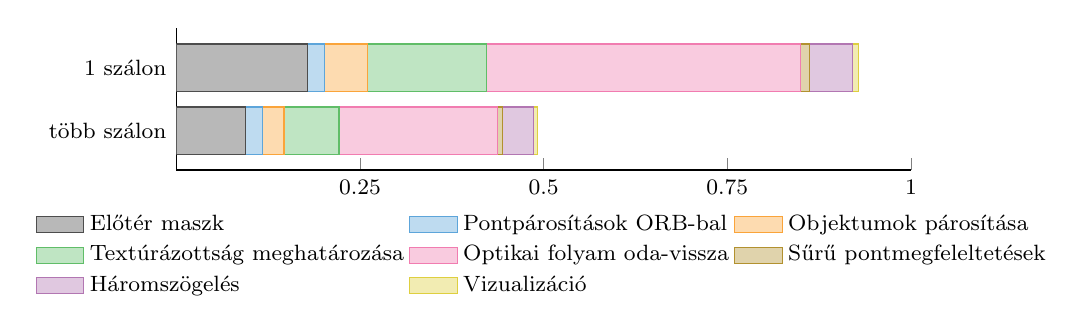
\begin{tikzpicture}
\begin{axis}[
    xbar stacked,
    legend style={
    legend columns=3,
        at={(xticklabel cs:0.5)},
        anchor=north,
        draw=none
    },
    ytick=data,
    axis y line*=none,
    axis x line*=bottom,
    tick label style={font=\footnotesize},
    legend style={font=\footnotesize},
    label style={font=\footnotesize},
    xtick={0.25, 0.5, 0.75, 1},
    width=.9\textwidth,
    bar width=6mm,
    xlabel={Idő másodpercben},
    yticklabels={1 szálon, több szálon},
    xmin=0,
    xmax=1,
    area legend,
    y=8mm,
    enlarge y limits={abs=0.625},
    legend cell align=left
]
\addplot[color1,fill=color1!40] coordinates {(0.178,1) (0.0944,0)};
\addplot[color2,fill=color2!40] coordinates {(0.0235,1) (0.0226,0)};
\addplot[color3,fill=color3!40] coordinates {(0.0583,1) (0.0296,0)};
\addplot[color4,fill=color4!40] coordinates {(0.163,1) (0.0749,0)};
\addplot[color5,fill=color5!40] coordinates {(0.427,1) (0.216,0)};
\addplot[color6,fill=color6!40] coordinates {(0.0119,1) (0.00618,0)};
\addplot[color7,fill=color7!40] coordinates {(0.0587,1) (0.042,0)};
\addplot[color8,fill=color8!40] coordinates {(0.00845,1) (0.0059,0)};

\legend{Előtér maszk, Pontpárosítások ORB-bal, Objektumok párosítása, Textúrázottság meghatározása, Optikai folyam oda-vissza, Sűrű pontmegfeleltetések, Háromszögelés, Vizualizáció}
\end{axis}  

\end{tikzpicture}
\caption{Első jelenet esetén az egyes lépések képkockánti átlagos időigénye másodpercben \label{fig:scene1_stats}}
\end{figure}

Ezekkel az apró javításokkal ellátva az alkalmazás kódját, \aref{table:result_scene1_multi}. táblázatban látható futási időket mértem az első jelenetre (itt még offline történt a feldolgozás, nem maradt ki egy képkocka sem). Az egyszálú végrehajtással összehasonlított átlagos idők \aref{fig:scene1_stats}. ábrán láthatóak. Megfigyelhető, hogy azon műveletek, amiket lehetett párhuzamosítani (pl. két képen ugyanazon művelet, két optikai folyam számolás), nagyjából kétszer gyorsabban fejeződtek be, a teljes folyamat pedig több, mint kétszeresére gyorsult. Ez annak köszönhető, hogy az objektumok rekonstrukcióit is párhuzamosítottam, valamint ebből következik az is, hogy egy teljes képkocka átlagos rekonstrukciója rövidebb ideig tart, mint a részfeladatok átlagainak szummája. Természetesen nem lehet a párhuzamosítással a végletekig menően gyorsítani, a rendelkezésre álló feldolgozóegységek korlátot szabnak az ésszerűen egymás mellett futtatható szálak számára, amely az én esetemben négy szál lett (ez pont ideális átlagosan két objektum/jelenet esetén).

\begin{table}[tbh]
\centering

\begin{tabular}{|l|l|l|l|l|}
\hline
\multirow{2}{*}{Tevékenység képkockánként} & \multicolumn{4}{ |c| }{Eltöltött idő (s)} \\\cline{2-5}
 & min & max & átlag & szórás \\ \hline\hline

Előtér maszk (2 kamerára) & 0,0875 & 0,103 & \textbf{0,0944} & 0,00261 \\\hline
Pontpárosítások ORB-bal & 0,0122 & 0,0368 & 0,0226 & 0,00347 \\\hline
Objektumok párosítása & 0,0206 & 0,0441 & 0,0296 & 0,00344 \\\hline

Textúrázottság meghatározása & 0,0208 & 0,11 & \textbf{0,0749} & 0,0153 \\\hline
Optikai folyam oda-vissza & 0,0731 & 0,312 & \textbf{0,216} & 0,0489 \\\hline
Sűrű pontmegfeleltetések & 0,000751 & 0,0122 & 0,00618 & 0,00147 \\\hline

Háromszögelés & 0,000567 & 0,058 & 0,042 & 0,0103 \\\hline
Vizualizáció & 0,00065 & 0,00838 & 0,0059 & 0,00138 \\
\hline \hline
Teljes folyamat & 0,109 & 0,574 & \textbf{0,391} & 0,105 \\ \hline

\end{tabular} 

\caption{Többszálú végrehajtás esetén az első jelenet feldolgozása során az egyes lépések futási idejükhöz kapcsolódó statisztikái (178 képkocka) \label{table:result_scene1_multi}}
\end{table}

%----------------------------------------------------------------------------
\section{Optikai folyam számolása GPU-n}
%----------------------------------------------------------------------------

OpenCV keretrendszerben néhány általam is használt eljárást a CUDA \cite{parallel-cuda} platformra is implementálták, melyeket egy külön \texttt{cv::cuda} névtéren belül találhatunk. Ezek segítségével, ha a videókártya támogatja, az algoritmusok implementációit a grafikus kártyán hatékonyabban futtathatjuk így növelve a teljesítményt.

\Aref{table:result_scene1_multi}. táblázatban láthatjuk, hogy az optikai folyam számolások, mind a sűrű pontmegfeleltetések számolásához, mind az előtér maszkhoz sok időt emésztenek fel. Miután feltelepítettem a CUDA Toolkit-et az NVIDIA honlapjáról \cite{cuda-nvidia}, újrafordítottam az OpenCV-t forrásból engedélyezve a CUDA modulokat. A GPU-s Färneback optikai folyam implementációját a \texttt{cv::cuda::FarnebackOpticalFlow} osztályban találtam meg. Ezzel a módosítással további jelentős sebességnövekedést értem el, mely statisztikáit \aref{table:result_scene1_multi_gpu}. táblázat mutatja. Ezzel a megoldással az első jeleneten kb. 4 FPS-es feldolgozási sebességet értem el.

Az ORB-bal történő jellegzetes pontok detektálása és leírók számolása is történhet a GPU-n, viszont tesztelések alapján úgy tűnt, hogy ezek a műveletek nem szálbiztosak. A dokumentáció \cite{cuda-stream} is említi, hogy némelyik függvény konstans GPU buffert használ, így ugyanazon műveletek egymás utáni többszöri meghívása okozhat problémákat (az előző optikai folyam számolása úgy tűnt nem ilyen -- konkrét dokumentációt erről nem találtam). Sebességben ez kb. 0,01 másodpercet jelentett volna képkockánként, annak kárára, hogy ezt a részt szálbiztossá teszem, így ezt az ötletet elvetettem.

\Aref{table:result_scene1_multi_gpu}. táblázatban jól látható, hogy jelenleg a legtöbb időt a textúrázottság meghatározása, valamint maga az optikai folyam kiszámolása viszi el. Utóbbin már nagyon nem lehet javítani, esetleg egy másik algoritmus választásával, előbbin pedig GPU-n történő számolással. Ezeket érdemes lenne a jövőben megvizsgálni.

\begin{table}[tbh]
\centering

\begin{tabular}{|l|l|l|l|l|}
\hline
\multirow{2}{*}{Tevékenység képkockánként} & \multicolumn{4}{ |c| }{Eltöltött idő (s)} \\\cline{2-5}
 & min & max & átlag & szórás \\ \hline\hline

Előtér maszk (2 kamerára) & 0,0304 & 0,0384 & \textbf{0,0337} & 0,00148 \\\hline
Pontpárosítások ORB-bal & 0,0176 & 0,0351 & 0,0262 & 0,00321 \\\hline
Objektumok párosítása & 0,0298 & 0,0477 & 0,0395 & 0,00328 \\\hline

Textúrázottság meghatározása & 0,0252 & 0,131 & 0,0886 & 0,0188 \\\hline
Optikai folyam oda-vissza & 0,0404 & 0,226 & \textbf{0,124} & 0,0405 \\\hline
Sűrű pontmegfeleltetések & 0,00101 & 0,0166 & 0,00773 & 0,00256 \\\hline

Háromszögelés & 0,000221 & 0,0561 & 0,0348 & 0,012 \\\hline
Vizualizáció & 0,00252 & 0,0106 & 0,00665 & 0,0016 \\
\hline \hline
Teljes folyamat & 0,137 & 0,338 & \textbf{0,259} & 0,0406 \\ \hline

\end{tabular} 

\caption{Többszálú végrehajtás és GPU-n történő optikai folyam számolás esetén az első jelenet feldolgozási statisztikája \label{table:result_scene1_multi_gpu}}
\end{table}

Megjegyzem, hogy az OpenCV-nek a még ki nem adott 3.0-s verziójától kezdve az OpenCL keretrendszerrel is jobb az integrációja \cite{amd-opencl-opencv}, és a dokumentáció alapján kicsiny befektetés mellett, lényegében transzparensen érhető el, hogy minden, amit felkészítettek rá az OpenCL kernelek segítségével párhuzamosan fusson heterogén rendszereken. Amint láthattuk a CUDA-s megvalósítás nem ilyen, ott explicit függvényhívásokkal kell operálnunk a megnövekedett teljesítmény eléréséhez. Az OpenCL egyik előnye az lenne, hogy a videókártya típusától függetlenül tudnánk kihasználni az ebben rejlő lehetőségeket. Nekem sajnos nem sikerült a gyakorlatban kipróbálnom az OpenCL-es újításokat, és a kódbázis még annyira friss, hogy a dokumentációban és az interneten sem találtam ehhez segítséget.


%----------------------------------------------------------------------------
\section{Valós idejű helyreállíthatóság vizsgálata}
%----------------------------------------------------------------------------

A következőkben megvizsgálom, hogy milyen feltételek mellett érhető el a megvalósított megoldással valós idejű helyreállítás az átalam használt számítógépen. Az alkalmazott kamerákból kinyert videofolyamok átlagosan 30 képkockát tartalmaznak másodpercenként. Mivel a televíziózásban és a mozi világában még mindig igen elterjedt a 24 FPS használata, így én is akkor tekintem valós idejűnek a feldolgozást, ha legalább 24 képkockát sikerül rekonstruálnom másodpercenként. Amennyiben meghaladom a 12 képkockát másodpercenként, akkor azt közel-valós idejűnek tekintem. A következőkben megvizsgálom, hogy mekkora felbontás, valamint képen látható objektum-méret esetén milyen sebesség érhető el.

Először a képkockák méretét próbáltam csökkenteni a \texttt{cv::resize()} függvénnyel két lépésben, először $320\times 240$-es, majd $160\times 120$-as felbontásra. A sebességre jótékony hatással volt a képméretek csökkenése, viszont a rekonstrukció minőségére éppen ellenkezőleg. Azokon a képkockákon, ahol az objektumok helyben forogtak, de vízszintes irányban nem sokat mozdultak értékelhetetlen lett a helyreállítás. Ez annak a következménye, hogy sok párosítás szempontjából fontos pont a kicsinyítés miatt eltűnt, illetve a képpontok eredeti mozgása a kisebb képeken elhanyagolható lett. Azonos képkockához tartozó rekonstrukciók eredményei és azok sebességei (csak azon képkockák feldolgozásai idejeit számolva, ahol ténylegesen sikerült helyreállítani legalább 1 objektumot) láthatóak \aref{fig:resize}. ábrán. Ezek alapján sajnos nem sikerült elérni a valós idejű feldolgozást, csak a közel-valós idejűt jelentős minőségcsökkenés és információsveszteség mellett.

\begin{figure}[tbh]
\centering
\begin{subfigure}[b]{.32\linewidth}
	\centering
	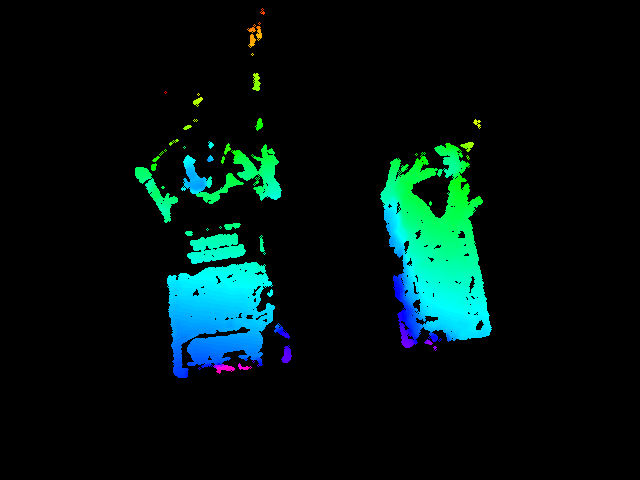
\includegraphics[width=137pt]{figures/vis_127_640.png}
	\caption{$640\times 480$; 3,86 FPS}
  \end{subfigure}
\begin{subfigure}[b]{.32\linewidth}
	\centering
	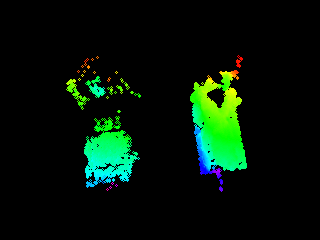
\includegraphics[width=137pt]{figures/vis_127_320.png}
	\caption{$320\times 240$; 10,1 FPS}
  \end{subfigure}
\begin{subfigure}[b]{.32\linewidth}
	\centering
	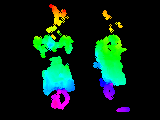
\includegraphics[width=137pt]{figures/vis_127_160.png}
	\caption{$160\times 120$; 14,3 FPS}
  \end{subfigure}
\caption{Egyre kisebb képkockák esetén a helyreállítás eredménye a bal oldali kamera nézőpontjából \label{fig:resize}}
\end{figure}

Ezt követően, a képkockák méretét nem kicsinyítéssel, hanem levágással csökkentettem. Az első jelenet esetében a képek érdemi része középen található, így először nagyjából középső $320\times 240$-es felbontású részt vettem figyelembe (mindegyik kamerán azt a részt, amelyen nagyjából ugyanaz a térrész látható). Ekkor átlagosan 7,35 FPS-es sebességet értem el, mely főleg annak köszönhető, hogy a kisebb méret miatt általában csak 1 objektum látszódott, így csak egyet kellett rekonstruálni. \Aref{fig:cut_320_240}. ábrán látható ugyanazon képkockáknak a helyreállított vizualizációi, mint \aref{fig:scene1_frames}. ábrán (\pageref{fig:scene1_frames}. oldal).

\begin{figure}[tbh]
\centering
\begin{subfigure}[b]{.32\linewidth}
	\centering
	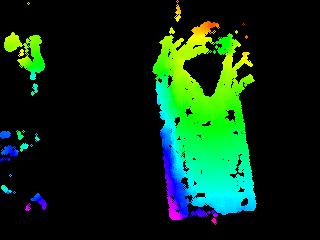
\includegraphics[width=137pt]{figures/vis_93_320.png}
  \end{subfigure}
\begin{subfigure}[b]{.32\linewidth}
	\centering
	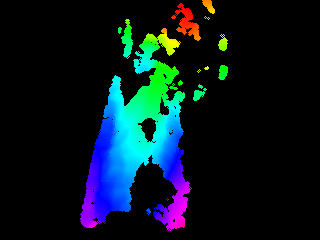
\includegraphics[width=137pt]{figures/vis_152_320.png}
  \end{subfigure}
\begin{subfigure}[b]{.32\linewidth}
	\centering
	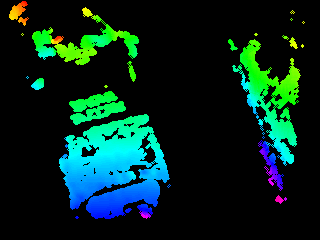
\includegraphics[width=137pt]{figures/vis_223_320.png}
  \end{subfigure}
\caption{Az első jelenet 40., 100. és 170. képkockájának a középső $320\times 240$-es képrészleteinek helyreállításai a bal oldai kamera nézőpontjából \label{fig:cut_320_240}}
\end{figure}

Ebből kiindulva az objektum detektálás implementációját lecseréltem a \texttt{SingleObjectSelector}-ra, valamint az objektumot a kamerától távolabb mozgattam, hogy kisebb területet foglaljon el, és a képeken az objektumot tartalmazó $160\times 140$-as területeket használtam a rekonstruáláshoz. Nagyjából minden második képkockánál volt értékelhető az eredmény, a kis objektum méret és a rendelkezésre álló területen történő kicsiny mozgás miatt. Időnként a maszk kijelölés nem sikerült jól, máskor pedig az előzetes ORB alapú párosítás volt helytelen, ami rossz optikai folyamot eredményezett. \Aref{fig:cut_160_140}. ábrán látható néhány egészen pontos rekonstrukció a két kamera képével és a két kamera közötti nézőpontból rekonstruált nézettel.

\begin{figure}[tbh]
\centering
\begin{subfigure}[b]{\linewidth}
	\centering
	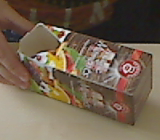
\includegraphics[width=137pt]{figures/tiny_vis_153_left.png}\hspace{5pt}
	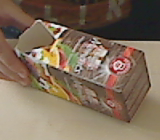
\includegraphics[width=137pt]{figures/tiny_vis_153_right.png}\hspace{5pt}
	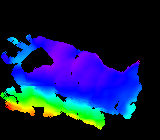
\includegraphics[width=137pt]{figures/tiny_vis_153.png}
	\caption{}
  \end{subfigure} \\\vspace{5pt}
  \begin{subfigure}[b]{\linewidth}
	\centering
	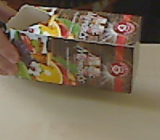
\includegraphics[width=137pt]{figures/tiny_vis_76_left.png}\hspace{5pt}
	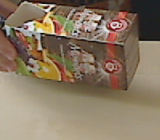
\includegraphics[width=137pt]{figures/tiny_vis_76_right.png}\hspace{5pt}
	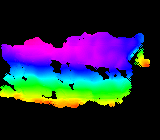
\includegraphics[width=137pt]{figures/tiny_vis_76.png}
	\caption{}
  \end{subfigure}
\caption{$160\times 140$-es felbontású képek és azok rekonstrukciói. A rekonstrukció a két kamera közötti képzeletbeli szakasz felezőpontjában vett nézőpontból készült \label{fig:cut_160_140}}
\end{figure}

Ilyen korlátok mellett éppen sikerült elérni a másodpercenkénti 12 képkocka rekonstrukcióját, ami az általam közel-valós idejű feldolgozásnak tekintett sebesség alsó határa. \Aref{table:cut_160_140}. táblázat mutatja az adott lépések hosszát. Átlagosan 5 pixel lett képkockánként az átlagos visszavetítési hiba, ami szintén a távoli objektum következtében jelentkező információhiánynak tudható be. A továbbiakban nem próbálkoztam még kisebb képeken az objektumok helyreállításával, mert már ezen utolsó feldolgozás hasznossága az alsó küszöböt érinti. Ennél kisebb információtartalommal rendelkező rekonstrukcióknak nincs gyakorlati haszna, még valós időben sem.

\begin{table}[b]
\centering

\begin{tabular}{|l|l|l|l|l|}
\hline
\multirow{2}{*}{Tevékenység képkockánként} & \multicolumn{4}{ |c| }{Eltöltött idő (s)} \\\cline{2-5}
 & min & max & átlag & szórás \\ \hline\hline

Előtér maszk (2 kamerára) & 0,0127 & 0,0425 & 0,0189 & 0,0055 \\\hline
Pontpárosítások ORB-bal & 0,00229 & 0,0216 & 0,0066 & 0,0031 \\\hline
Objektumok párosítása & 0,00555 & 0,129 & 0,0188 & 0,0112 \\\hline

Textúrázottság meghatározása & 0,00117 & 0,0352 & 0,0158 & 0,00562 \\\hline
Optikai folyam oda-vissza & 0,00239 & 0,0485 & 0,0222 & 0,00548 \\\hline
Sűrű pontmegfeleltetések & 0,000649 & 0,0161 & 0,00284 & 0,00292 \\\hline

Háromszögelés & 0,00001 & 0,0188 & 0,00434 & 0,00427 \\\hline
Vizualizáció & 0,000257 & 0,00776 & 0,00106 & 0,000901 \\
\hline \hline
Teljes folyamat & 0,0184 & 0,206 & \textbf{0,083} & 0,0263 \\ \hline

\end{tabular} 

\caption{$160\times 140$-es felbontású képek rekonstrukciói során az egyes lépések átlagos hosszai (230 képkocka) \label{table:cut_160_140}}
\end{table}


%----------------------------------------------------------------------------
\section{Összefoglaló}
%----------------------------------------------------------------------------

Ebben a fejezetben bemutattam, hogy az implementáció sebességét milyen megközelítések mentén tudtam javítani. Kitértem az OpenMP segítségével megvalósított párhuzamosításra, valamint az OpenCV-ben támogatott CUDA platform használatára. A fejezet végén pedig a valós idejű helyreállíthatóságot és ennek korlátait vizsgáltam meg. Ennek során arra jutottam, hogy az elkészült megoldással szigorúan vett valós idejű rekonstrukció nem valósítható meg az általam használt hardveren, ellenben kvázi-valós idejű igen, amennyiben kis méretű (\textasciitilde $150\times 150$) objektumot kell detektálni és helyreállítani a videofolyamok alapján.
